\documentclass{article}
\usepackage{amsmath}
\usepackage{amssymb}
\usepackage[a4paper, top=25mm, bottom=25mm, left=25mm, right=25mm]{geometry}
\usepackage{pgfplots}
\usepackage{mathtools}
\pgfplotsset{compat=1.18}

\begin{document}
\pagestyle{empty}
\large

\begin{center}
2011-2012 Spring \\MAT123-[Instructor] Midterm II\\(08/05/2012)\\Time: 15:00 - 16:45\\Duration: 105 minutes
\end{center}

\noindent 1. Consider the region bounded by the curve $y=x^2$, the $x$-axis, and the line $x=2$, where $x\geq0$.

\hfill

(a) Find the volume of the solid generated by revolving the region about the $x$-axis by the disk method and sketch the solid.

\hfill

(b) Find the volume of the solid generated by revolving the region about the $y$-axis by the shell method and sketch the solid.

\hfill

\noindent 2. Evaluate the following integrals.

\hfill

(a) $\displaystyle \int_0^3\left|x^2-1\right|\, dx$ \ \ \ (b) $\displaystyle\int\frac1{x^2+2x+1}\,dx$ \ \ \ (c) $\displaystyle\int\frac1{x^2+2x+2}\,dx$

\hfill

\hfill

(d) $\displaystyle\int\frac1{x^2+3x+2}\,dx$ \ \ \ (e) $\displaystyle\int_{-\pi/6}^0\sqrt{1-\cos(6x)}\,dx$

\hfill

\noindent 3. Determine whether the improper integral $\displaystyle\int_{-\infty}^\infty\frac1{1+x^2}\,dx$ is convergent or divergent. Evaluate if the integral is convergent.

\hfill

\noindent 4. Evaluate the following limits. Explain all your work and write clearly.

\hfill

(a) $\displaystyle\lim_{x\to0}\frac{3^x-1}{5^x-1}$ \ \ \ (b) $\displaystyle \lim_{x\to0}\frac{\displaystyle\int_0^{x^2}\sin t\,dt}x$

\hfill

\noindent 5. Determine whether each sequence converges or diverges. Evaluate the limit of each convergent sequence. Explain all your work and write clearly.

\hfill

(a) $\displaystyle a_n=\frac{2n+(-1)^n}n$ \ \ \ (b) $\displaystyle a_n=\arctan\left(\frac{n+1}n\right)$ \ \ \ (c) $\displaystyle a_n = \frac{n+1}{1-\sqrt n}$


\newpage

\begin{center}
2011-2012 Spring Midterm II (08/05/2012) Solutions\\
(Last update: 29/08/2025 20:11)
\end{center}

\noindent 1.
\begin{center}
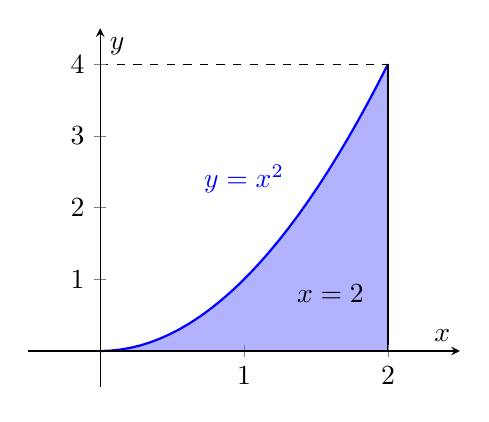
\begin{tikzpicture}
  \begin{axis}[
    axis lines=middle,
    xmin=-0.5, xmax=2.5,
    ymin=-0.5, ymax=4.5,
    xtick={0,1,2},
    ytick={0,1,2,3,4},
    xlabel=$x$, ylabel=$y$,
    domain=0:2,
    samples=30,
    axis on top,
    clip=true,
    scale=0.8,
    ]
    
    \addplot [
      draw=none,
      fill=blue!30,
    ]
    {x^2}
    \closedcycle;

    \addplot [thick, blue] {x^2};

    \draw (axis cs:2,0) -- (axis cs:2,4);
    \draw[dashed] (axis cs:0,4) -- (axis cs:2,4);
    \node[blue] at (1,2.4) {$y=x^2$};
    \node at (1.6,0.8) {$x=2$};
   \end{axis}
\end{tikzpicture}
\end{center}

\hfill

\noindent (a)
\begin{center}
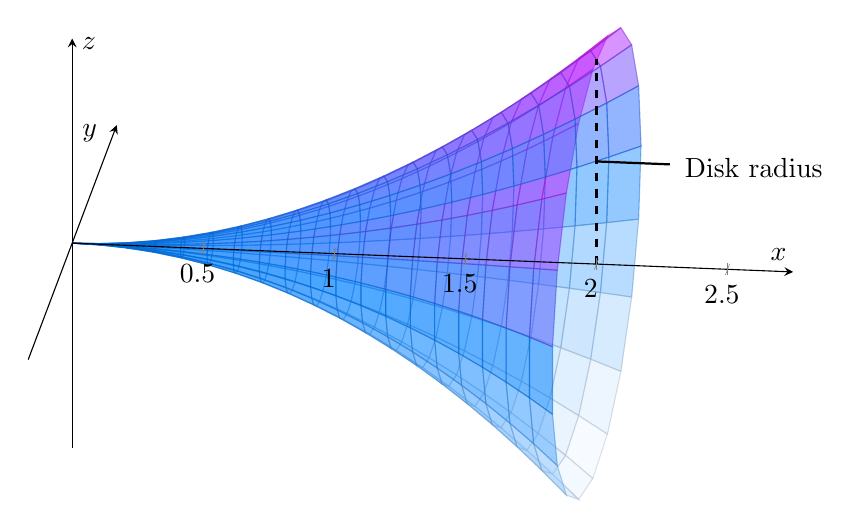
\begin{tikzpicture}
  \begin{axis}[
    view={7}{30},
    axis on top,
    axis lines=middle,
    xlabel={$x$},
    ylabel={$y$},
    zlabel={$z$},
    ytick={-4,4}, ztick={-4,4},
    samples=20,
    xmin=0, xmax=2.75,
    domain=0:2,
    y domain=0:360,
    colormap/cool,
    scale=1.5,
    ytick=\empty, ztick=\empty
    ]
    
    \addplot3 [
      surf,
      opacity=0.5,
    ]
    (
      x,
      {x^2 * cos(y)},
      {x^2 * sin(y)}
    );

    \draw[dashed, thick] (2,0,0)--(2,0,4);
    \draw[thick] (2,0,2)--(2.28,0,2);

    \node at (2.6,0,2) {Disk radius};
  \end{axis}
\end{tikzpicture}
\end{center}
\begin{align*}
\text{Volume}&=\int_{\mathcal{D}}\pi\cdot(r(x))^2\,dx=\int_0^2\pi\left(x^2\right)^2\,dx=\pi\int_0^2x^4\,dx=\pi\left[\frac{x^5}5\right]_0^2=\boxed{\frac{32\pi}5}
\end{align*}

\hfill

\noindent (b)
\begin{center}
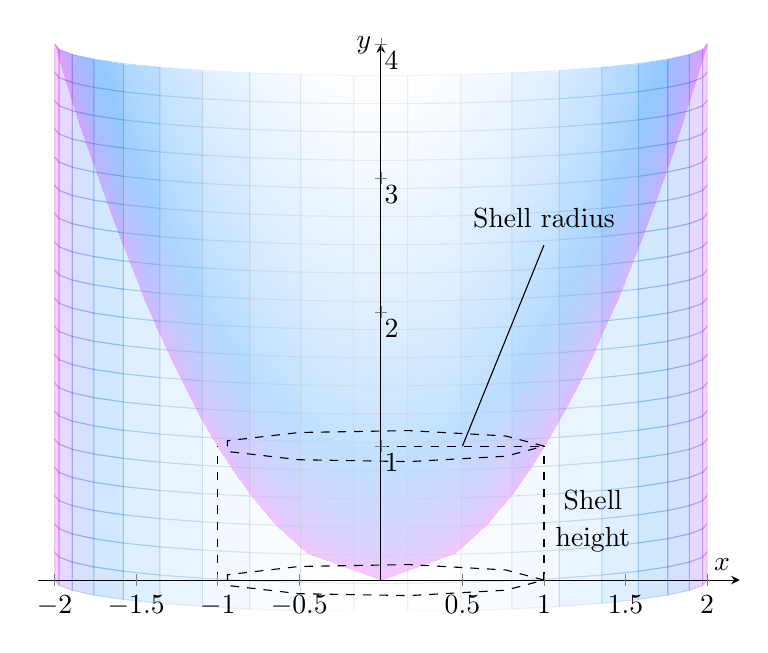
\begin{tikzpicture}
  \begin{axis}[
  view={0}{85},
    axis lines=center,
    axis on top,
    xlabel={$x$},
    ylabel={$y$},
    zlabel={$z$},
    hide z axis,
    xmin=-2.1, xmax=2.2,
    samples=20,
    domain=0:4,
    y domain=180:360,
    colormap/cool,
    scale=1.3,
    ]

    \addplot3 [
      surf,
      opacity=0.3,
      shader=interp,
    ]
    (
      {sqrt(x) * cos(y)},
      {x},
      {sqrt(x) * sin(y)}
    );
    
    \addplot3[
      surf,
      opacity=0.2,
    ]
    (
      {2 * cos(y)},
      {x},
      {2 * sin(y)}
    );

    \addplot3[
      domain=0:360,
      samples=10,
      dashed,
    ]
    (
      {cos(x)},
      {1},
      {sin(x)}
    );
    
    \addplot3[
      domain=0:360,
      samples=10,
      dashed,
    ]
    (
      {cos(x)},
      {0},
      {sin(x)}
    );
    \draw[dashed] (1,0,0)--(1,1,0);
    \draw[dashed] (-1,0,0)--(-1,1,0);
    \draw[dashed] (0,1,0)--(1,1,0);
    \draw (0.5,1,0)--(1,2.5,0);
    \node at (1.3,0.6,0) {Shell};
    \node at (1.3,0.3,0) {height};
    \node at (1,2.7,0) {Shell radius};
  \end{axis}
\end{tikzpicture}
\end{center}
\begin{align*}
\text{Volume}&=\int_{\mathcal{D}}2\pi\cdot r(x)\cdot h(x)\,dx=2\pi\int_0^2x\cdot x^2\,dx=2\pi\int_0^2x^3\,dx\\\\&=2\pi\left[\frac{x^4}4\right]_0^2=2\pi\left(\frac{2^4}4-0\right)=\boxed{8\pi}
\end{align*}

\noindent 2. 

\hfill

\noindent (a) The expression $\left|x^2-1\right|$ is the same as $x^2-1$ for $x>1$ and $1-x^2$ for $x<1$. We can write the equivalent expression below.

\begin{align*}\int_0^3\left|x^2-1\right|&=\,dx\int_0^1\left(1-x^2\right)\,dx+\int_1^3(x^2-1)\,dx=\left[x-\frac{x^3}3\right]_0^1+\left[\frac{x^3}3-x\right]_1^3\\\\&=\left[\left(1-\frac{1^3}3\right)-0\right]+\left[\left(\frac{3^3}3-3\right)-\left(\frac{1^3}3-1\right)\right]=\boxed{\frac{22}3}\end{align*}

\hfill

\noindent (b)
\begin{align*}\int\frac1{x^2+2x+1}\,dx=\int\frac1{(x+1)^2}\,dx=\boxed{-\frac1{x+1}+c, \quad c\in\mathbb{R}}\end{align*}

\hfill

\noindent (c)
\begin{align*}\int\frac1{x^2+2x+2}\,dx&=\int\frac1{(x+1)^2+1}\,dx\quad\left[u=x+1\implies du=dx\right]\\\\&=\int\frac1{u^2+1}\,du=\arctan(u)+c=\boxed{\arctan(x+1) +c,\quad c\in\mathbb{R}}\end{align*}

\hfill

\noindent (d) We can use the method of partial fraction decomposition.

\begin{equation}\int\frac1{x^2+3x+2}\,dx=\int\frac1{(x+1)(x+2)}\,dx=\int\left(\frac A{x+1}+\frac B{x+2}\right)\,dx\end{equation}

\begin{align*}
A(x+2)+B(x+1)&=1\\
x(A+B)+2A+B&=1\\
\therefore A+B=0\quad[\text{eliminate}\ x]\,&\rightarrow\,2A+B=1
\end{align*}

\[
\left.
\begin{array}{ll}
A+B=0\\
\displaystyle2A+B=1
\end{array}
\right\}
\quad A=1,\quad B=-1
\]

\hfill

\noindent Plug the values of $A$ and $B$ into $(1)$.

\begin{equation*}\int\left(\frac A{x+1}+\frac B{x+2}\right)\,dx=\int\left(\frac1{x+1}-\frac1{x+2}\right)\,dx=\boxed{\ln\left|x+1\right|-\ln\left|x+2\right|+c,\quad c\in\mathbb{R}}\end{equation*}

\hfill

\noindent (e) Use the trigonometric identity $\cos(2x)=1-2\sin^2x$.

\begin{equation*}\int_{-\pi/6}^0\sqrt{1-\cos(6x)}\,dx=\int_{-\pi/6}^0\sqrt{2\sin^2(3x)}\,dx=\sqrt2\int_{-\pi/6}^0\left|\sin(3x)\right|\,dx\end{equation*}

\hfill

\noindent $\sin x<0$ for $-\pi<x<\pi$. Therefore, the integral can be rewritten as follows.

\begin{align*}\sqrt2\int_{-\pi/6}^0\left|\sin(3x)\right|\,dx&=\sqrt2\int_{-\pi/6}^0-\sin(3x)\,dx=\sqrt2\left[\frac13\cos(3x)\right]_{-\pi/6}^0\\\\&=\frac{\sqrt2}3\left[\cos0-\cos\left(-\frac\pi2\right)\right]=\boxed{\frac{\sqrt2}3}\end{align*}

\hfill

\noindent 3. We have an improper integral where the limits are $\pm\infty$. Use limits to handle improper integrals accurately.

\begin{align*}
\int_{-\infty}^\infty\frac1{1+x^2}\,dx&=\lim_{A\to\infty}\int_{-A}^A\frac1{1+x^2}\,dx = \lim_{A\to\infty}\arctan(x)\bigg|_{-A}^A\\\\&=\lim_{A\to\infty}\left(\arctan A-\arctan(-A)\right)=\frac\pi2-\left(-\frac\pi2\right)=\boxed\pi
\end{align*}

\hfill

\noindent The value of the improper integral is finite. Therefore, this integral is convergent.

\hfill

\noindent 4.

\hfill

\noindent (a) The limit is in the indeterminate form $0/0$. We can apply L'Hôpital's rule to eliminate the indeterminate form.

\[\lim_{x\to0}\frac{3^x-1}{5^x-1}\overset{\text{L'H.}}{=}\lim_{x\to0}\frac{3^x\cdot\ln3}{5^x\cdot\ln5}=\log_53\cdot\lim_{x\to0}\left(\frac35\right)^x=\boxed{\log_53}\]

\hfill

\noindent (b) The first method is to evaluate the integral in the limit.

\[\lim_{x\to0}\frac{\displaystyle\int_0^{x^2}\sin t\,dt}x=\lim_{x\to0} \frac{-\cos t\,\bigg|_{t=0}^{t=x^2}}x=\lim_{x\to0}\frac{-\cos x^2-(-\cos0)}x=\lim_{x\to0}\frac{1-\cos x^2}x\]

\hfill

\noindent Multiply by the expression inside the limit $\displaystyle \frac xx$. Notice that we obtain a standard form.

\begin{align*}\lim_{x\to0}\left(\frac{1-\cos x^2}x\cdot\frac xx\right)&=\lim_{x\to0}\frac{1-\cos x^2}{x^2}\cdot\lim_{x\to0}x\quad\left[\lim_{u\to0}\frac{1-\cos u}u = 0\right]\\\\&=0\cdot0=\boxed0\end{align*}

\hfill

\noindent The second method is to use L'Hôpital's rule because of the $0/0$ form.

\[\lim_{x\to0}\frac{\displaystyle\int_0^{x^2}\sin t\,dt}x\overset{\text{L'H.}}{=}\lim_{x\to0}\frac{\displaystyle\frac d{dx}\int_0^{x^2}\sin t\,dt}1\]

\hfill

\noindent Let $u=x^2$, then $du=2x\,dx$. By the Fundamental Theorem of Calculus, the limit can be rewritten as follows.

\[\lim_{x\to0}\displaystyle\frac d{dx}\int_0^{x^2}\sin t\,dt=\lim_{x\to0}\frac d{du}\left(\int_0^u\sin t\,dt\right)\frac{du}{dx}=\lim_{x\to0}\left(\sin u\cdot 2x\right)=\lim_{x\to0}\left[2x\sin \left(x^2\right)\right]=\boxed0\]

\hfill

\noindent 5.

\hfill

\noindent (a)
\[a_n=\frac{2n+(-1)^n}{n}=2+\frac{(-1)^n}n\]

\hfill

\noindent The sequence converges to $\boxed2$ because $\displaystyle\frac{(-1)^n}n\to 0$ as $n\to\infty$.

\hfill

\noindent (b) $\arctan$ is continuous everywhere. Therefore, we can take the limit inside the expression.

\[\lim_{n\to\infty}\arctan\left(\frac{n+1}n\right)=\arctan\lim_{n\to\infty}\left(1+\frac1n\right)=\arctan1=\frac\pi4\]

\hfill

\noindent The sequence converges to $\displaystyle\boxed{\frac\pi4}$.

\hfill

\noindent (c)
\[\lim_{n\to\infty}\frac{n+1}{1-\sqrt n}=\lim_{n\to\infty}\frac{\sqrt n\left(\sqrt n+\frac1{\sqrt n}\right)}{\sqrt n\left(\frac1{\sqrt n}-1\right)}=\lim_{n\to\infty}\frac{\sqrt n+\frac1{\sqrt n}}{\frac1{\sqrt n}-1}=-\infty\]

\hfill

\noindent Notice that the denominator approaches $-1$ as $n\to\infty$ and the numerator approaches $\infty$ as $n\to\infty$. The sequence diverges to $\boxed{-\infty}$.

\end{document}